%!TEX root = main.tex

\section{Numerical solutions}
\label{sec:numerics}
\subsection{Equilibrium branch identification}

We now switch to the study of  the nonlinear regime  and we will resort to numerical calculations  to explore the system's behavior beyond the linear approximation\comment[id=ALB]{Let's clarify our use of linear/nonlinear}.

In order to find the equilibrium branches we make use of a pseudo-arclength continuation technique implemented in the software AUTO~\cite{Doedel1981-sa}. It solves the nonlinear equation Eqs. \ref{auto1} or  \ref{auto2} in the case of rigid and non-rigid foundations, respectively, with the relative end displacement $\bar\epsilon$ treated as a continuation parameter. To discretize the boundary-value problem, it uses collocation with Lagrange polynomials, and in our simulations, we had $N=300$ mesh points with $N_c = 5$ collocation nodes and activated mesh adaptation. 
\begin{figure}
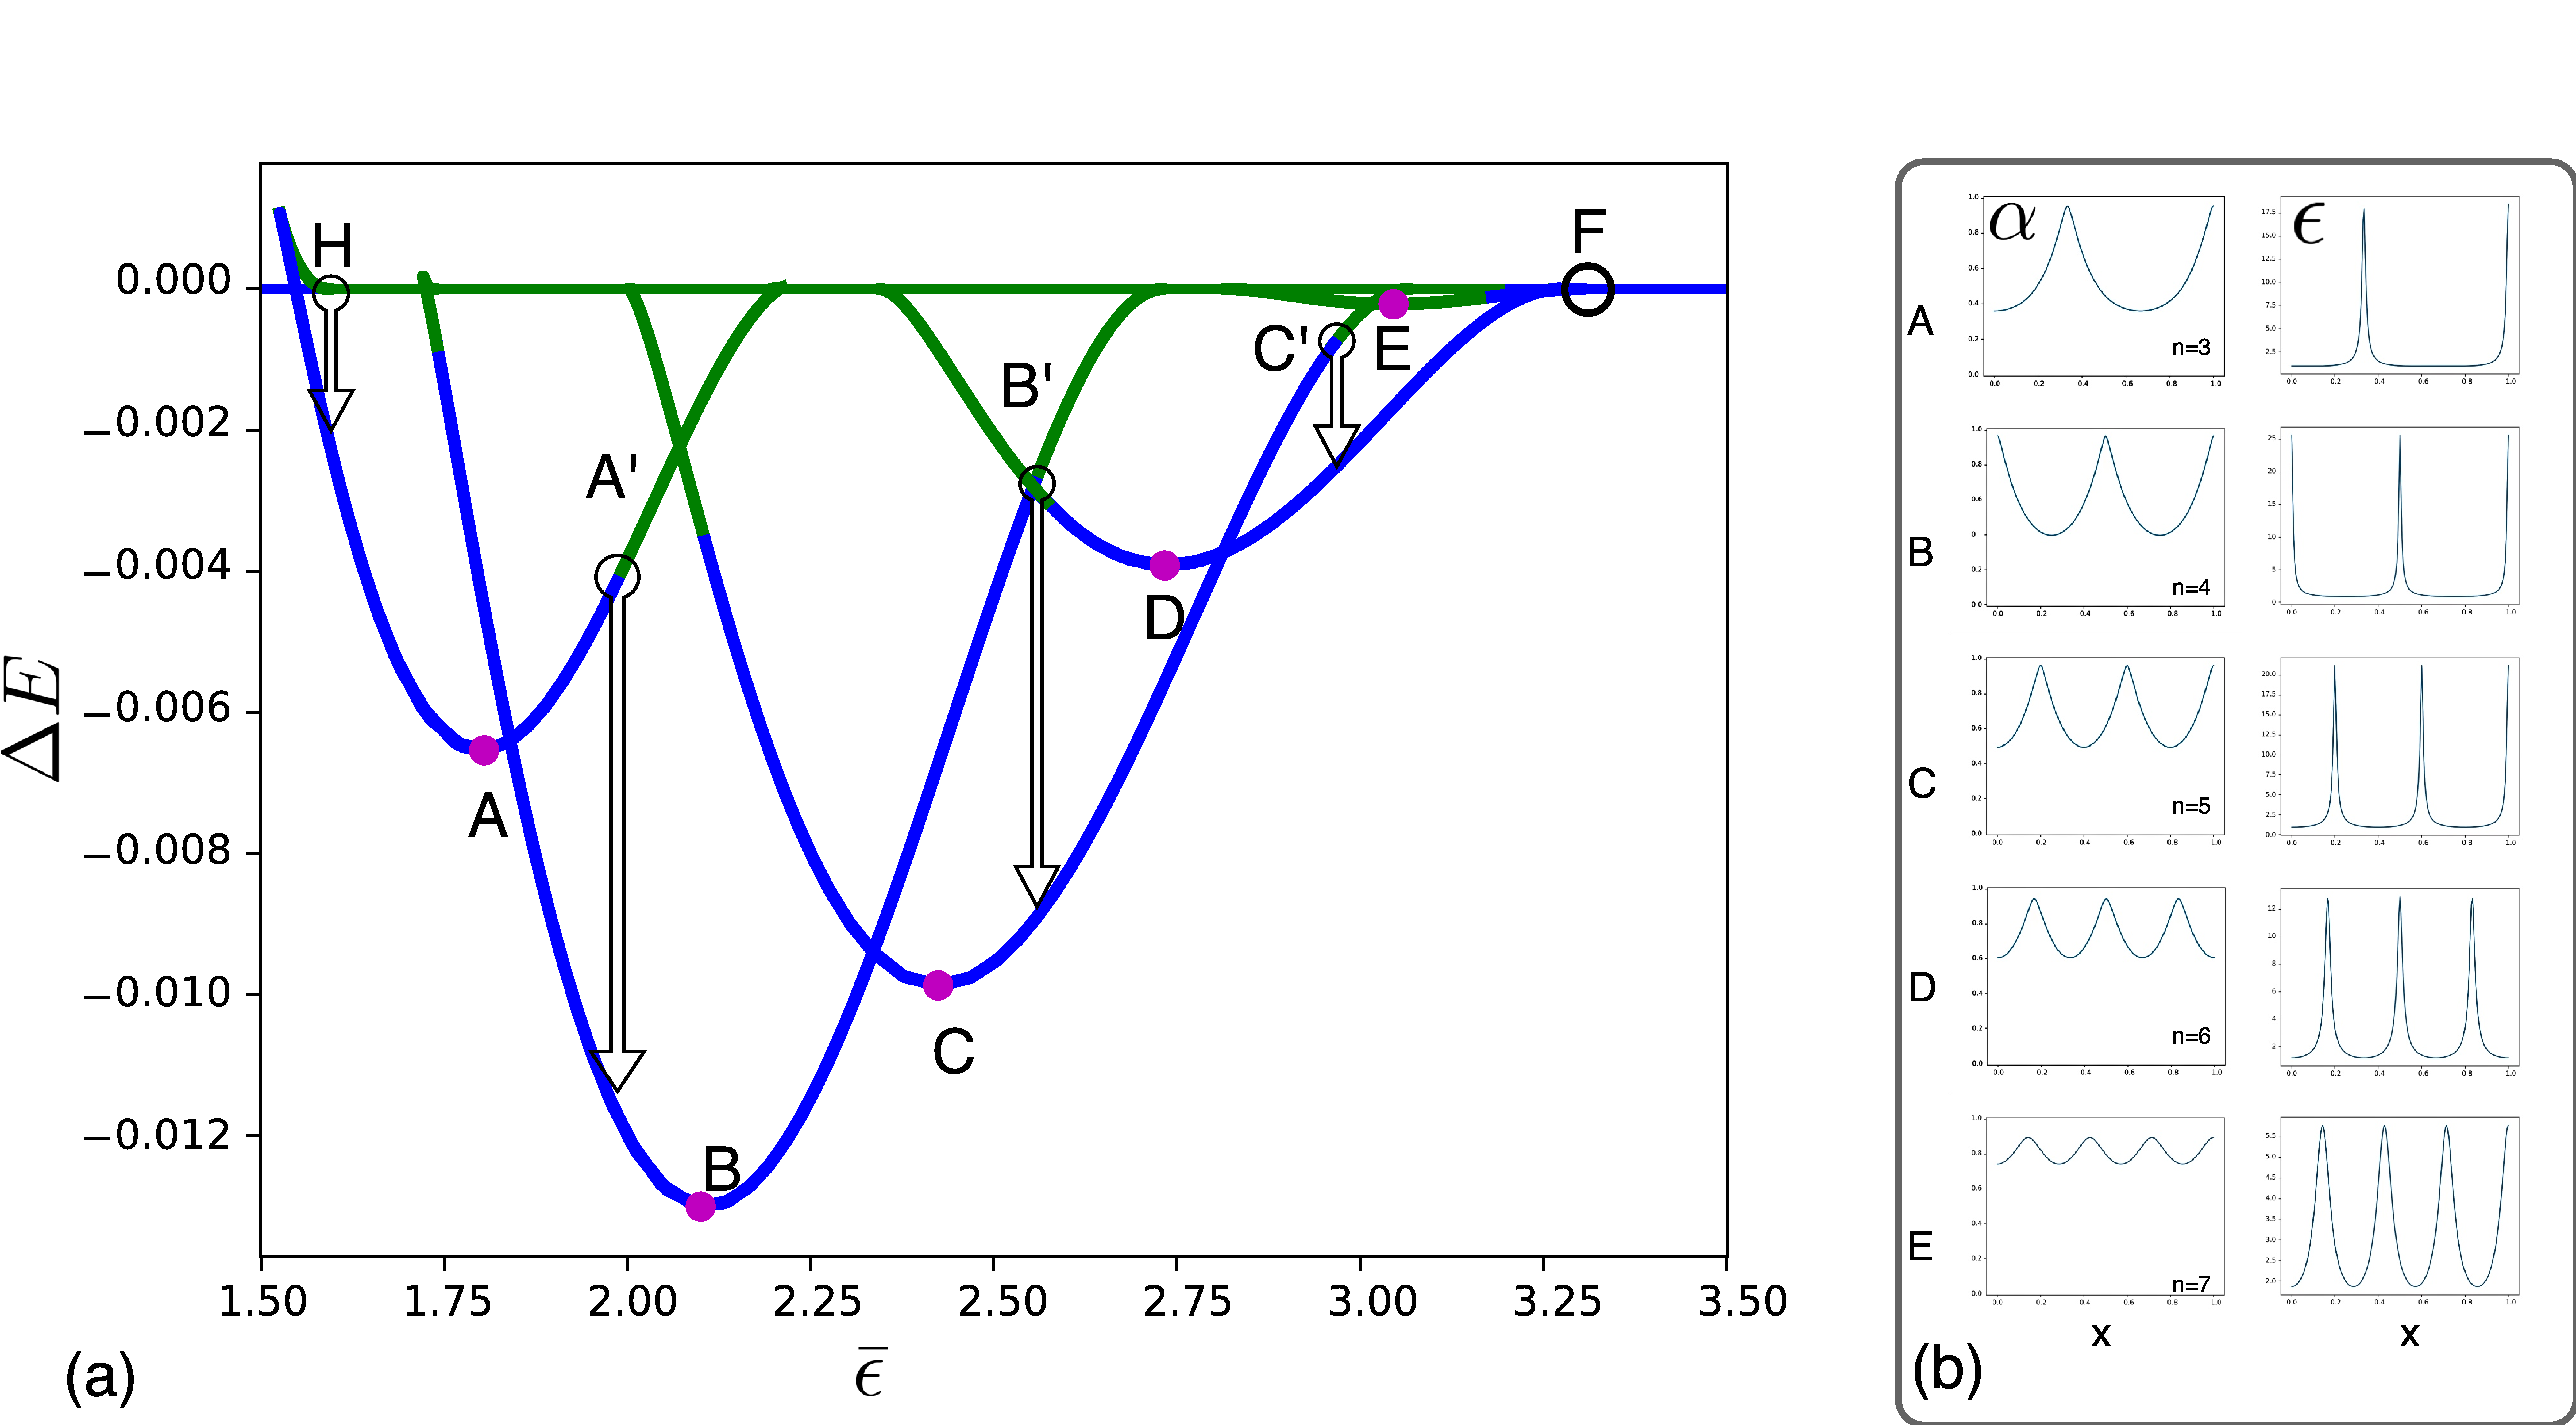
\includegraphics[scale=0.1]{./final_images/fig2.pdf}
    \caption{
\todo[inline]{Add marker for $\ep_c$ in a), }
Equilibrium branches in the phase-field model of an elastic bar on rigid elastic foundation: (a) the energy difference $\Delta E$ between the affine and non-affine configurations. Stability of solutions is indicated by colors: blue denotes stability, while green indicates instability   via the numerical evaluation of the smallest eigenvalue of the stiffness matrix $\mathbf{K}^1$. Arrows indicate the anticipated branch switching events associated with the loss of stability; (b) the damage and strain profiles of the minimum energy configurations on each branch.}
    \label{fig:enter-label}
\end{figure}
In order to asses the stability of equilibrium branches, we use  the numerical evaluation of the smallest eigenvalue of the second variation by discretizing the integrals \eqref{hessian22} and   \eqref{hessian222} to construct the stiffness matrix
${\bf K}$ and investigating numerically the sign of the minimal eigenvalue $\kappa$ of the corresponding finite quadratic form \cite{Sanderson2016-ht}.  The finite element discretization of the displacement and damage field $(u, \alpha )$     with \( n_u \) displacement degrees-of-freedom 
$
\mathbf{u} = \{ u_1, \ldots, u_{n_u} \}^T 
$
and \( n_\alpha \) damage degrees-of-freedom 
$
\boldsymbol{\alpha} = \{ \alpha_1, \ldots, \alpha_{n_\alpha} \}^T.
$ are given by 
$
u(\mathbf{x}) \approx u_{\text{FE}} (\mathbf{x}) := \sum_{i=1}^{n_u} \mathcal{N}^{(u)}_i(\mathbf{x}) u_i $
and $\alpha(\mathbf{x}) \approx \alpha_{\text{FE}} (\mathbf{x}) := \sum_{i=1}^{n_\alpha} \mathcal{N}^{(\alpha)}_i (\mathbf{x}) \alpha_i 
$
where $\mathcal{N}^{(u)}(\mathbf{x}) $ and $\mathcal{N}^{(\alpha)}(\mathbf{x}) $ are the finite element basis functions and  $u_h$ and  $\alpha_h$ are nodal values for the displacement and damage fields, respectively. We used quadratic one-dimensional finite elements with 3 nodes  whose   shape functions   ${\mathcal N}_i(x)$ at a node $i$  are given by ${\mathcal N}_1(\xi)=-0.5\xi(1-\xi)$, ${\mathcal N}_2(\xi)=-0.5\xi(1+\xi)$ and ${\mathcal N}_3(\xi)=-(1-\xi)(1+\xi)$, where $\xi$ is the isoparameteric coordinate. The discrete solution $u(x_i)$ provided at discrete nodes $x_i$ by AUTO was first interpolated using B-spline basis functions of degree 3 \cite{Grimstad2016-cq}, and then utilized to calculate the integrals \eqref{hessian22} and   \ref{hessian222} employing a three-point Gauss integration scheme. The fixed boundary conditions were enforced by removing the rows and columns corresponding to $x = 0$ and $x = 1$ from the stiffness \added[id=ALB]{sub-} matrix $\mathbf{K}$\added[id=ALB]{$\mathbf K^i_{uu}$ for $i=1, 2$}. The explicit form of the stiffness matrix for the first model is given by  
\begin{equation}
{\bf K}^1=\begin{bmatrix}
\int_0^1[ \frac{1}{\lambda_2^2}{\mathcal N}_i{\mathcal N}_j + (1-\alpha)^2{\mathcal N}'_i{\mathcal N}'_j
%+\frac{1}{\lambda_2^2}{\mathcal N}_i {\mathcal N}_j
] dx&
-2\int_0^1(1-\alpha)u' {\mathcal N}'_i {\mathcal N}_j  dx\\
-2\int_0^1(1-\alpha)u' {\mathcal N}_i {\mathcal N}'_j dx
& \int_0^1 [ (2+u'^2){\mathcal N}_i{\mathcal N}_j +\lambda_1^2{\mathcal N}'_i{\mathcal N}'_j] dx
\end{bmatrix},
\label{eq:stifness1}
\end{equation}
and in the second model it reads

\begin{equation}
{\bf K}^2=\begin{bmatrix}
\int_0^1[ \frac{1}{\lambda_2^2}{\mathcal N}_i{\mathcal N}_j + (1-\alpha)^2{\mathcal N}'_i{\mathcal N}'_j] dx&
-2\int_0^1(1-\alpha)u' {\mathcal N}'_i {\mathcal N}_j  dx&
-\int_0^1[\frac{1}{\lambda_2^2}{\mathcal N}_i {\mathcal N}_j]  dx\\

-2\int_0^1(1-\alpha)u' {\mathcal N}_i {\mathcal N}'_j dx&
 \int_0^1 [ (2+u'^2){\mathcal N}_i{\mathcal N}_j +\lambda_1^2{\mathcal N}'_i{\mathcal N}'_j] dx&
 0\\

-\int_0^1[\frac{1}{\lambda_2^2}{\mathcal N}_i{\mathcal N}_j ] dx
&0
&\int_0^1\frac{1}{\lambda_2^2}{\mathcal N}_i {\mathcal N}_j+r_s{\mathcal N}'_i {\mathcal N}'_j  dx
\end{bmatrix}.
\label{eq:stifness2}
\end{equation}
Our objective is to establish a branch switching strategy as part of our model's dynamic expansion. This extension must ensure the system's re-stabilization following an instability in a dissipative manner. Furthermore, in a quasi-static scenario, it should involve the selection of a new locally stable equilibrium branch with inherently lower energy.  Considering applications in structural mechanics, our approach to selecting the new equilibrium branch should involve utilizing the local energy minimizing (LEM)\comment[id=ALB]{Acronyms, imho, make it harder to read by requiring extra mental buffer.} criterion, which emulates the zero viscosity limit of overdamped viscous dynamics. This approach disregards the global energy minimizing (GEM) strategy, which may be relevant in biomechanical applications~\cite{Salman2021-mn}. According to LEM protocol, during quasi-static loading, the system will remain in a metastable state (a local minimum of energy) until it becomes unstable. Subsequently, during an isolated switching event, the new equilibrium branch will be chosen using a descent algorithm \cite{Puglisi2005-lg}.
\begin{figure}
    %\centering
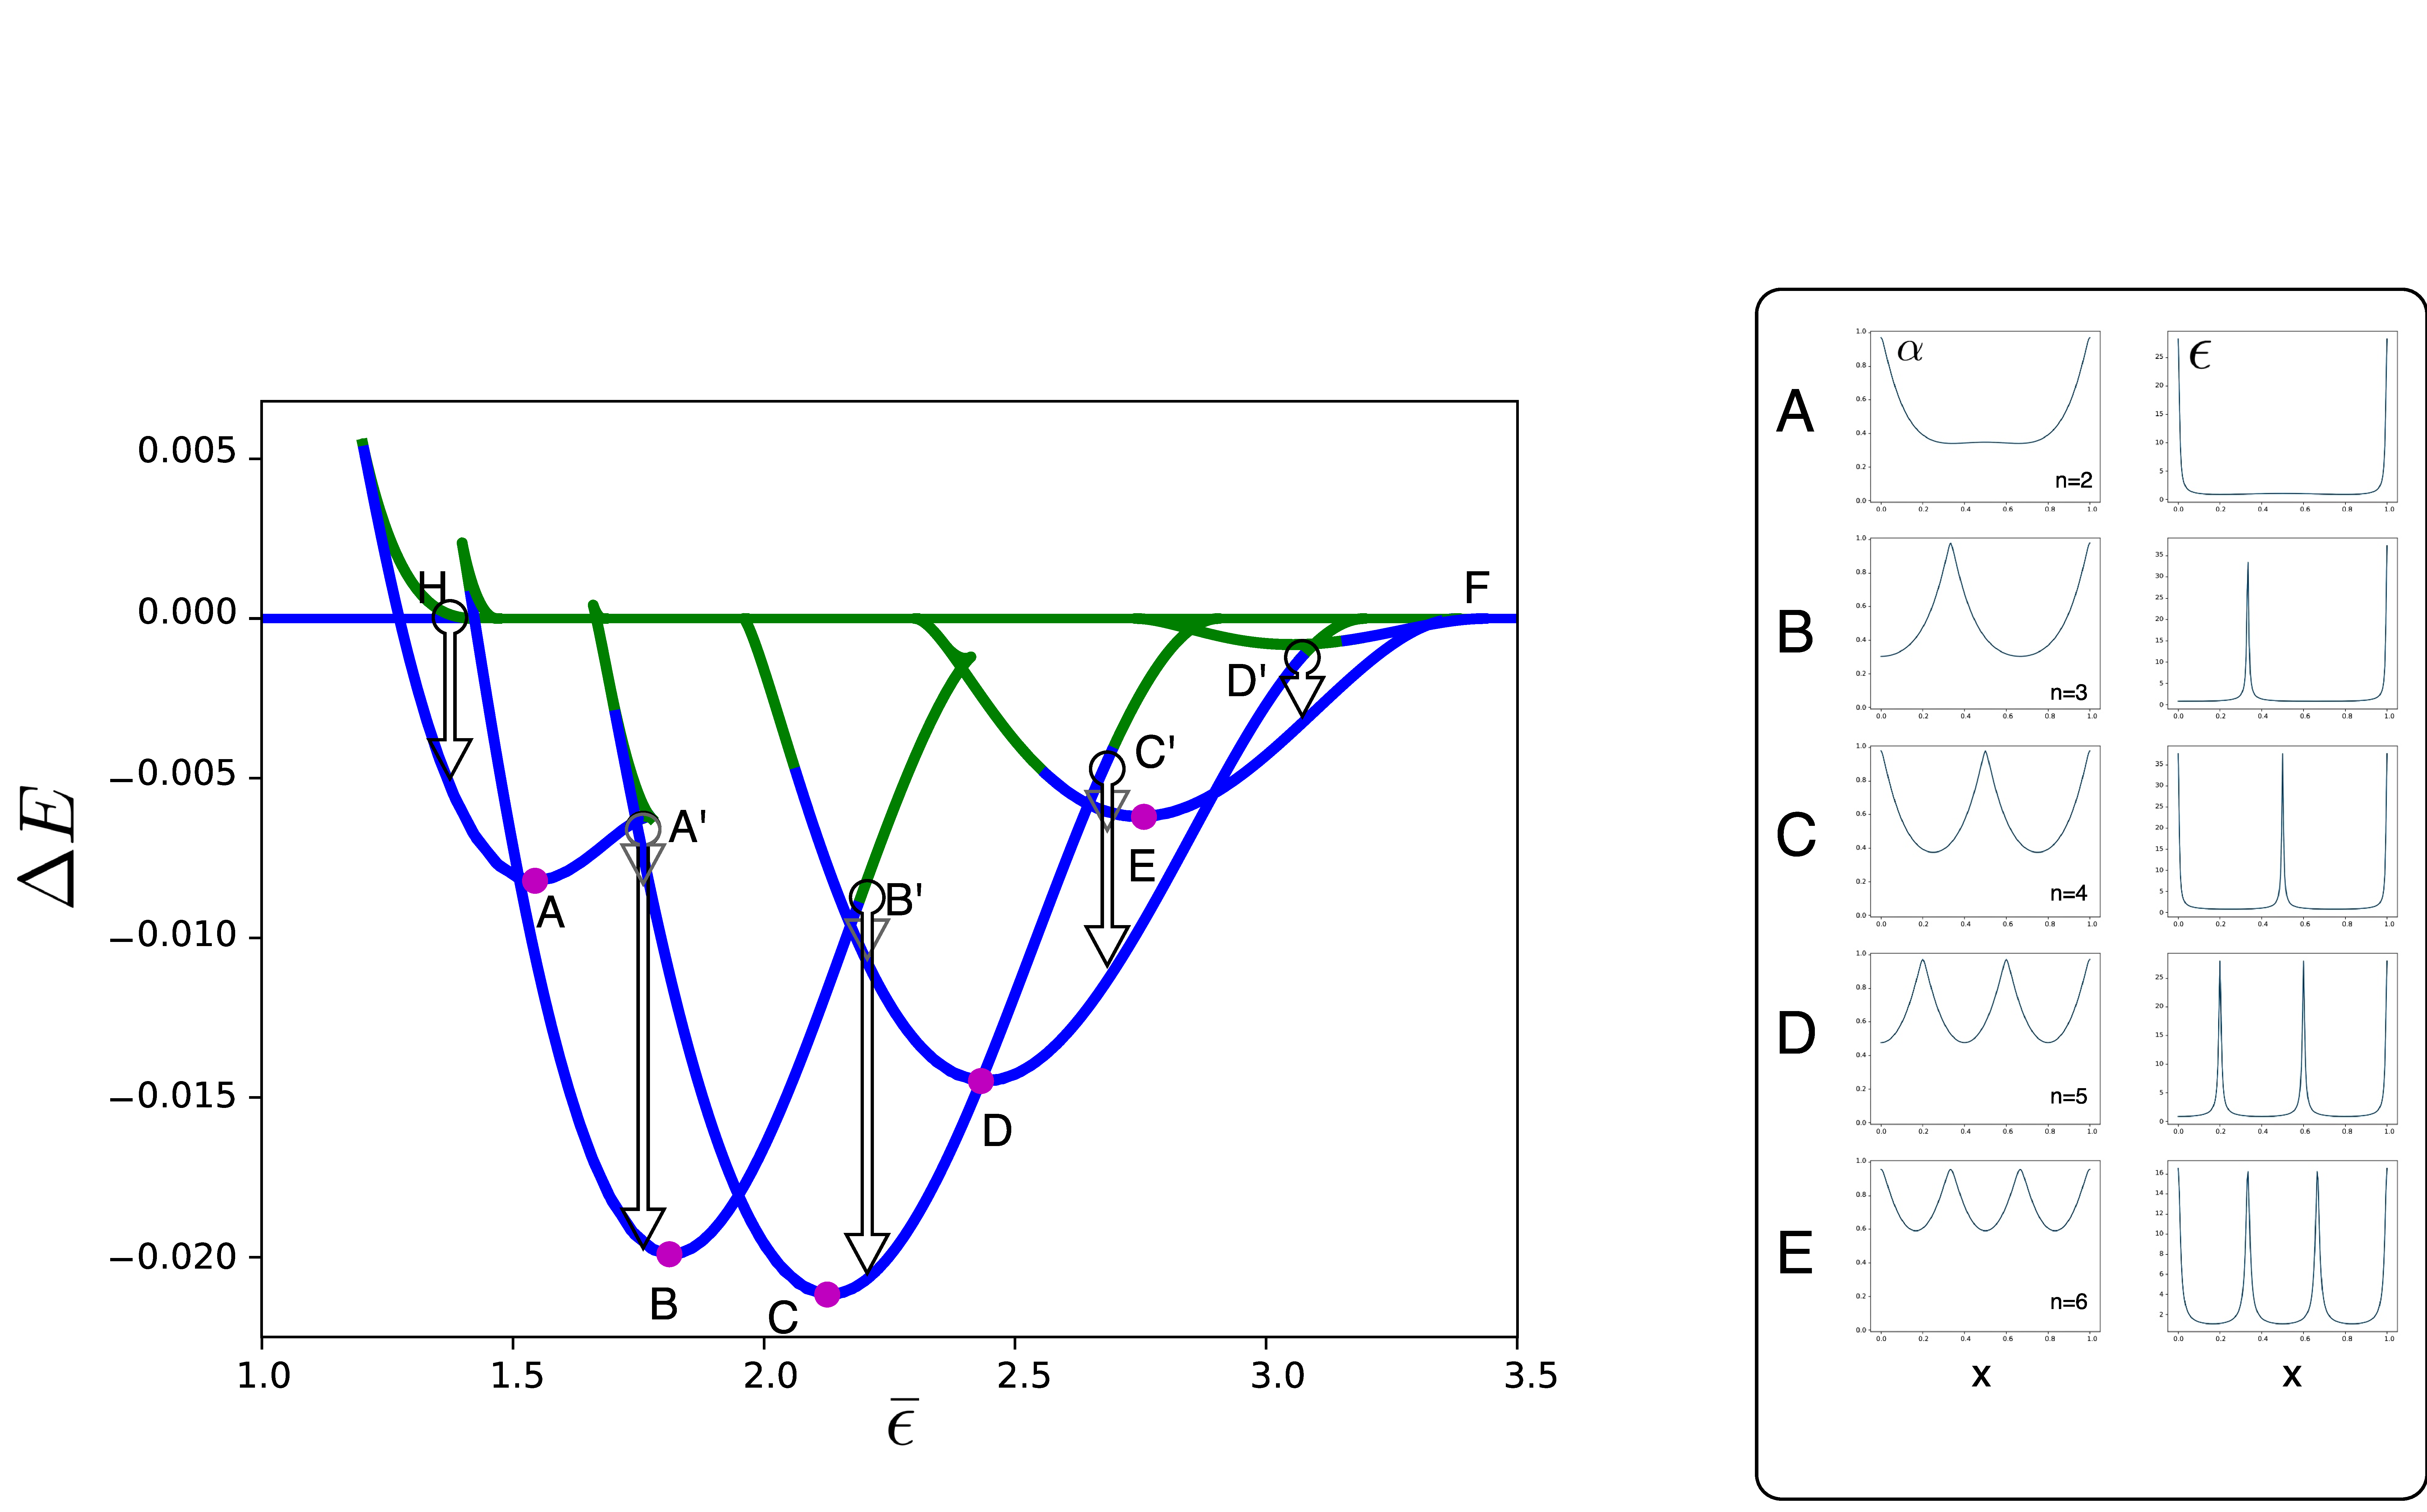
\includegraphics[scale=0.1]{./final_images/fig3.pdf}
    \caption{
\todo[inline]{
    Add marker for $\ep_c, H$ in Fig (a)
    Add marker for $n=1, 2, ...$ in Fig (a)
    }
Equilibrium branches in the phase-field model of an elastic bar on non-rigid elastic foundation: (a) the energy difference $\Delta E$ between the affine and non-affine configurations. Stability of solutions is indicated by colors: blue denotes stability, while green indicates instability   via the numerical evaluation of the smallest eigenvalue of the stiffness matrix $\mathbf{K}^2$; (b) the damage and strain profiles of the minimum energy configurations on each branch.}
    \label{fig:enter-label2}
\end{figure}

We display the equilibrium branches that solve the nonlinear equations (Eq. \ref{auto1}) in Fig. \ref{fig:enter-label}. These branches are characterized by plotting the energy difference $\Delta E$, which represents the energy difference between the energy of the current non-affine solution and the energy of the affine solution $f^0(\bar{\epsilon}, \alpha^0(\bar{\epsilon}))$ at the current value of the loading parameter $\bar\epsilon$. The stability of solutions is indicated by blue and green colors, representing stable and unstable solutions, respectively. Stability is discerned through numerical evaluation of the smallest eigenvalue denoted as $\kappa$ of the stiffness matrix $\mathbf{K}^1$, as defined in \eqref{eq:stifness1}.

Under the LEM protocol, the system remains on the trivial branch where the homogeneous solution remains stable until $\bar\epsilon^c$, identified using linear stability analysis. At the critical load $\bar\epsilon^c$  at the point H, following the first instability, a branch switching transition occurs from the trivial branch with $n = 0$ to the nontrivial equilibrium branch with $n = 3$, and the ensuing non-affine configuration is linearly stable, as seen in Fig. \ref{fig:enter-label}. We depict the lowest energy configuration on this equilibrium branch in Fig. \ref{fig:enter-label} at point A, consisting of two simultaneously nucleated localized cracks, one inside the domain and one on the boundary. 

When the loading parameter $\bar{\epsilon}$ is further increased, the equilibrium configuration with $n=3$ loses linear stability at point $A'$. In Fig. \ref{fig:enter-label}, it can be observed that under the LEM protocol, the only available transition from point $A'$ is to the branch with $n=4$, which remains locally stable within the corresponding range of applied strains $\bar{\epsilon}$. The minimum energy configuration on the branch with $n=4$ is depicted in Fig. \ref{fig:enter-label} at point $B$, consisting of two cracks: one inside the domain and two on the right and left boundaries.

At point $B'$, the stability of the branch with $n=4$ is lost, indicating a single available transition leading to the branch with $n=5$ (depicted by the black arrow). While the branch with $n=6$ appears accessible due to its lower energy compared to the current state, it is indeed unstable at the current  value of $\bar\epsilon$. The lowest energy configurations on the branches with $n=5$ and $n=6$ are illustrated in Fig. \ref{fig:enter-label}(C-D). From the branch with $n=5$, which loses linear stability at point $C'$, a branch switching event will occur to the branch with $n=7$,  the corresponding minimum energy configuration on this branch is depicted in Fig. \ref{fig:enter-label}(b). Finally, this branch reconnects to the trivial branch with $n=0$ at point $F$.

In the case of the second model, the equilibrium branches that solve the nonlinear equations (Eq. \ref{auto2}) are shown in Fig. \ref{fig:enter-label2}. We again plot the energy difference $\Delta E$, which represents the energy difference between the energy of the current non-affine solution and the energy of the affine solution $f^0(\bar{\epsilon}, \alpha^0(\bar{\epsilon}))$ at the current value of the loading parameter $\bar\epsilon$, to characterize thesxe branches. The stability of solutions is indicated by blue and green colors, representing stable and unstable solutions, respectively. Stability is now discerned through numerical evaluation of the smallest eigenvalue of the stiffness matrix $\mathbf{K}^2$, as defined in \eqref{eq:stifness2}.

We revisit the LEM protocol, where the initial transition from the trivial solution to the only available branch with $n=2$ occurs at $\epsilon_c^*$, marked as point H. Illustrated in Fig. \ref{fig:enter-label2}(b), the damage and strain profiles of the lowest energy configuration at point A reveal two boundary cracks. The $n=2$ branch concludes at point $A'$, a scenario absent in the initial model, leading to instability. However, the system can now access to two equilibrium branches: $n=3$ and $n=4$ shown in gray and black arrows. Fig. \ref{fig:enter-label2}(b) showcases the lowest energy configurations on these branches. The former (point B) comprises one bulk crack and one boundary crack, while the latter  (point C) exhibits one bulk crack and two boundary cracks. 

The choice of the subsequent branch at point $A'$ will dictate the ensuing crack growth. On both branches with $n=3$ and $n=4$, at the next instability points $B'$ and $C'$, the system will once again encounter two available equilibrium branches. Remaining on the $n=3$ branch, it can transition to either the $n=4$ or $n=5$ branch at point $B'$. Opting for the $n=4$ branch, the subsequent branch selection occurs at point $C'$, offering branches with $n=6$ or $n=5$. Notably, the $n=5$ branch smoothly reconnects with the trivial solution at point $F$. However, the $n=6$ branch experiences another branch selection event at point $D'$ before rejoining the trivial solution. 

Finally, we can conclude that  the overall behavior of the second model   reveals additional complexity with more branch switching events. In the first model, the LEM strategy revals a single path before reconnecting to the trivial branch, while in the second model, the system can follow 8 different paths. This additional complexity provides a good case to test numerical optimization methods, which we will discuss in the following.

\subsection{Equilibrium branch selection in overdamped viscous dynamic}
We consider now the equilibrium solutions reachable through the line-search based quasi-Newton algorithms such as  conjugate gradient or the BFGS optimization, which are effectively  mimics the zero viscosity limit of an overdamped viscous dynamics~\cite{SALMAN2012219}. Quasi-Newton methods serve as alternatives to Newton's method for locating roots or local extrema of functions. Particularly advantageous in scenarios where computing the Hessian at each iteration is impractical or computationally expensive, these methods circumvent the need for explicit Hessian computation. Instead, they rely on evaluating the function value and its gradient, updating the Hessian by analyzing successive gradient vectors.

Quasi-Newton methods are highly suitable for solving the phase-field equation of fracture, particularly when compared to standard Newton method-based monolithic solvers. Such solvers, which simultaneously  solve the equations for both damage and displacement variables, often falter when confronted with non-convex energy functionals. For example, as demonstrated in \cite{Wick2017-bo}, the Newton method-based monolithic algorithm does not consistently handle brittle fracture scenarios involving abrupt crack propagation. Recently, quasi-Newton methods, particularly the BFGS variant, have been employed to effectively solve the system of coupled governing equations in a monolithic fashion within the phase-field method of fracture. These methods have demonstrated success in various engineering applications, as evidenced by \cite{Kristensen2020-zy,Wu2020-qk,Salman2021-mn,Liu2022-ix}.

In  this study, it is worth to note that our primary objective is not to provide a comprehensive assessment of quasi-Newton methods on a global scale. Instead, our focus lies in scrutinizing their behavior and performance specifically concerning equilibrium branch selections within our simplified framework, where all branches are readily identified. By narrowing our scope to this specific aspect, we aim to gain insights into the effectiveness and reliability of quasi-Newton methods in reaching the equilibrium states of our system.
\begin{figure}
    %\centering
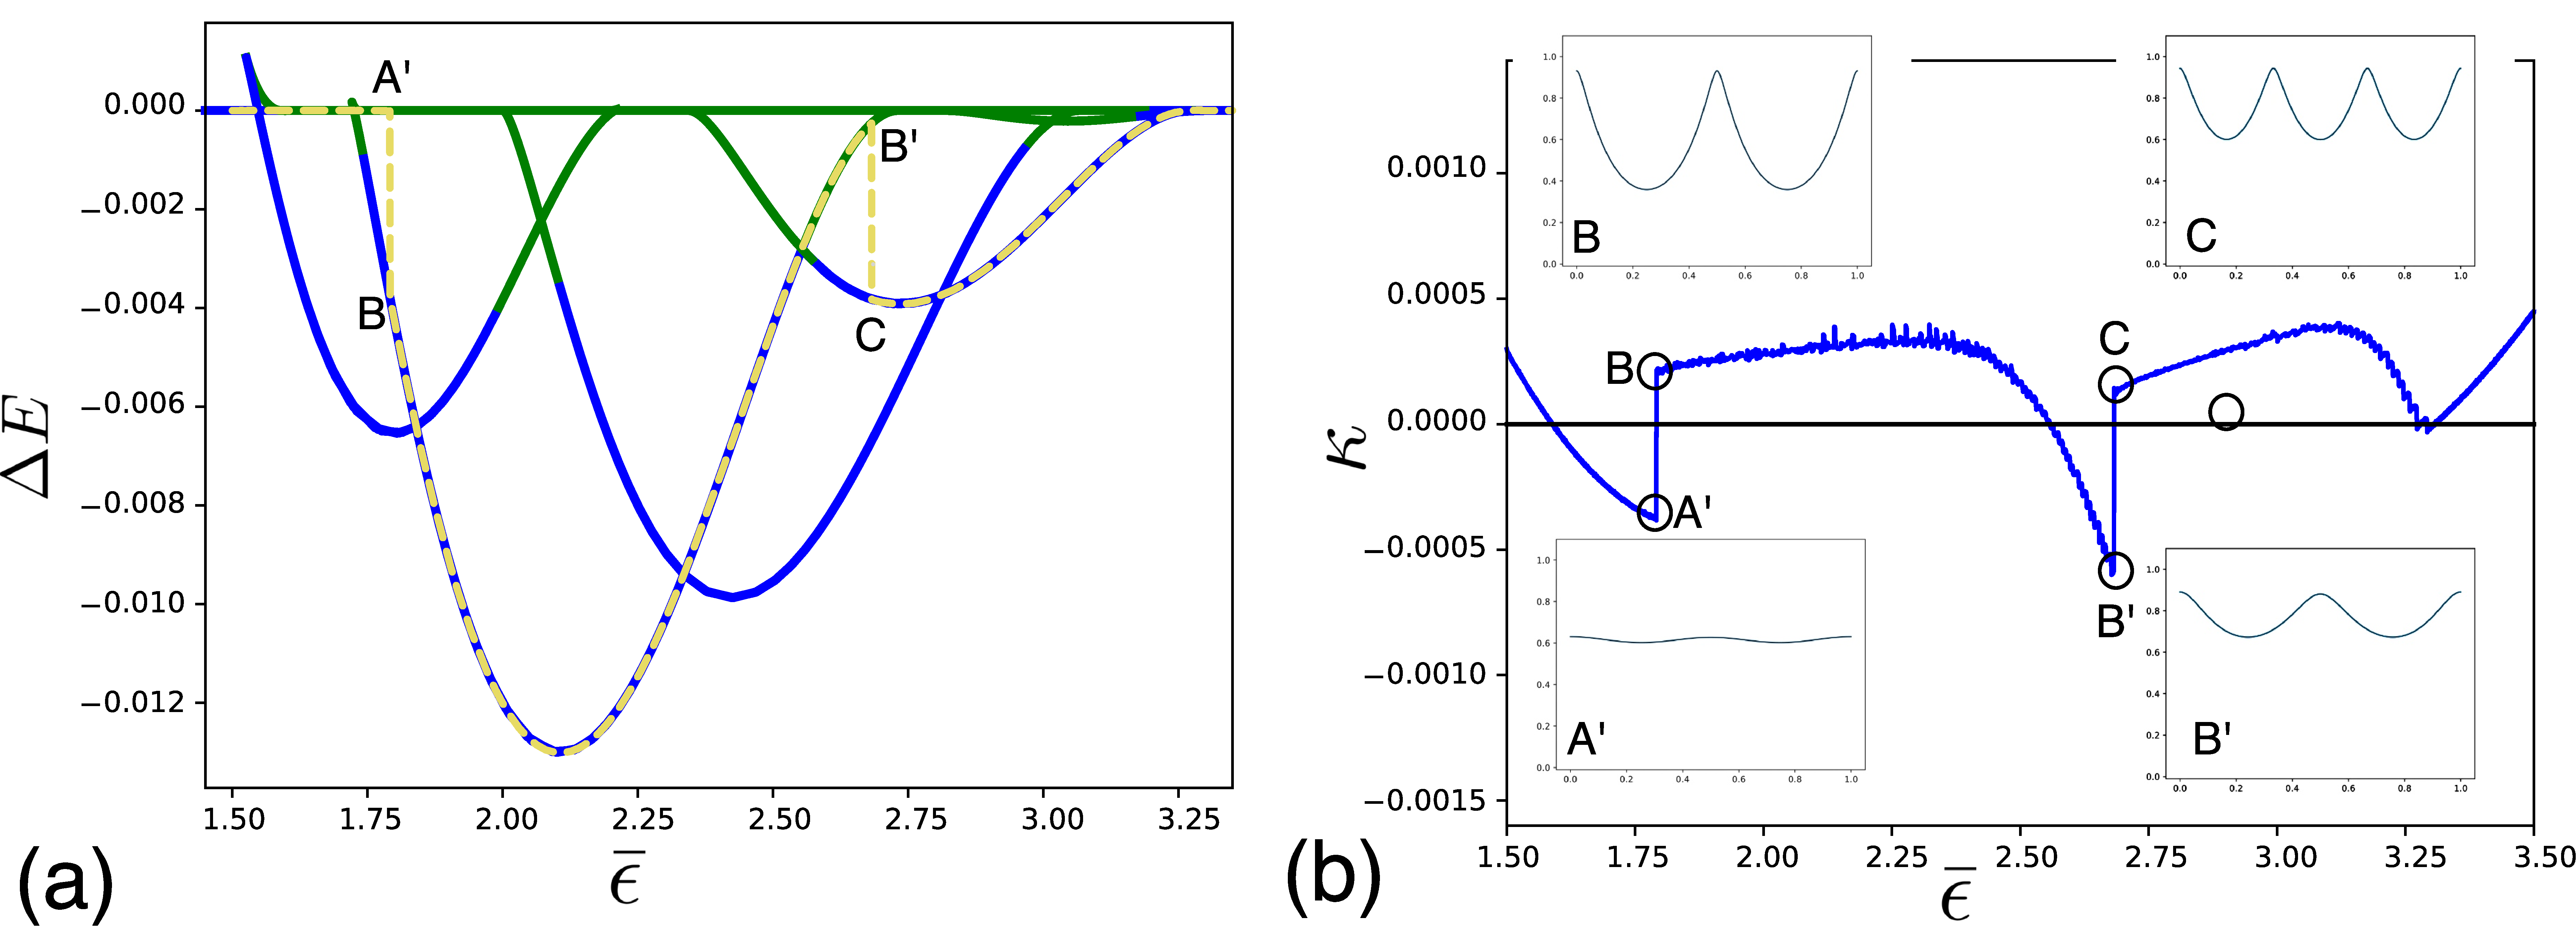
\includegraphics[scale=0.13]{./final_images/fig4.pdf}
    \caption{
\todo[inline]{Add marker for $\ep_c, H$ in Fig (a) and (b)}
Quasi-static loading simulations with L-BFGS: (a) the energy difference $\Delta E$, between he quasi-Newton solutions (gray dashed line) and the homogeneous solutions are superimposed onto equilibrium branches (red); (b) smallest eigenvalue of the second variation  as a function of the loading parameter $\bar\epsilon$; inset show damage profiles.}
    \label{fig:tempo1}
\end{figure}

To proceed further, we recall that quasi-Newton algorithms only evaluate the function value and its gradient to reach equilibrium configurations. This implies that in our case, we need to evaluate integrals \eqref{modeld} and \eqref{model_elastic_substrate}, along with their first variations given by \eqref{firstvar1} and \eqref{firstvar}, in the first and second models, respectively. We   discretized the integrals \eqref{firstvar1} and \eqref{firstvar} to construct the residuals vectors using finite elements to obtain 
\begin{equation}
{\bf R}^1=\int_0^1 [(1-\alpha)^2u'\mathcal{N}'_i+\frac{1}{\lambda_2^2} (u-u_0) \mathcal{N}_i+\frac{1}{2}(u'^2 g'(\alpha)+h'(\alpha))\mathcal{N}_i+\lambda_1^2\alpha'\mathcal{N}'_i ]dx,\label{residual1}
\end{equation}
in the first model and 
\begin{equation}
{\bf R}^2=\int_0^1 [(1-\alpha)^2u'\mathcal{N}'_i+\frac{1}{\lambda_2^2} (u-u_s) \mathcal{N}_i+\frac{1}{2}(u'^2 g'(\alpha)+h'(\alpha))\mathcal{N}_i+\lambda_1^2\alpha'\mathcal{N}'_i +r_su_s'\mathcal{N}_i]dx\label{residual2}.
\end{equation}
in the second model. 

Among iterative methods for large-scale unconstrained optimization, particularly when dealing with possibly dense Hessian matrices,  quasi-Newton methods often emerge as preferable alternatives to the widely-used Newton-Raphson (NR) algorithm. The NR algorithm, conventionally utilized for solving linear equations to determine the correction $\Delta \mathbf{X}^{(k)}$ from the current estimate $\mathbf{X}^{(k)} = (\mathbf{u}^{(k)}, \boldsymbol{\alpha}^{(k)})$ at iteration $k$, is expressed in our context as:
\begin{equation}
K_{ij} \Delta X_j + R_i = 0,
\label{Eq:NR}
\end{equation}
where the discrete stiffness matrix $\mathbf{K}$ and bulk forces $\mathbf{R}$ are initialized with the initial guess $\mathbf{X}^{(k)}$. Subsequently, the guess is updated as $\mathbf{X}^{(k+1)} = \mathbf{X}^{(k)} + \Delta \mathbf{X}^{(k)}$ after solving Equation \eqref{Eq:NR} using LU factorization~\cite{Sanderson2016-ht}. It's evident that the NR algorithm fails if the discrete stiffness matrix $\mathbf{K}$ isn't invertible.


On the other hand, quasi-Newton methods, as well-established (see standard textbooks, e.g., \cite{Nocedal1999-zr,Nocedal2006-qh}), they generate a sequence $\left\{\mathbf{X}^{(k)}\right\}$ according to the following scheme:
\begin{equation}
\mathbf{X}^{(k+1)} = \mathbf{X}^{(k)} + h^{(k)} \mathbf{p} ^{(k)}, \quad k=0,1,\ldots
\end{equation}
with
\begin{equation}
\mathbf{p}^{(k)}=-(\mathbf{B}^{(k)})^{-1}{\bf R},
\end{equation}
where $(\mathbf{B}^{(k)})^{-1}$ approximates the inverse of the Hessian matrix  $\mathbf{K}$ and $h^{(k)}$ represents a step length. Particularly, instead of computing $(\mathbf{B}^{(k)})^{-1}$  at each iteration $k$, these methods update $(\mathbf{B}^{(k)})^{-1}$ in a straightforward manner to obtain the new approximation $(\mathbf{B}^{(k+1)})^{-1}$  for the subsequent iteration. Additionally, rather than storing full dense $n \times n$ approximations, they only retain a few vectors of length $n$, enabling implicit representation of the approximations. Moreover, the choice of the step length $h^{(k)}$ is carried out through a line search to minimize a function $f(h^{(k)}) = f(\mathbf{X}^{(k)} + h^{(k)} \mathbf{p}^{(k)})$ in order to find an acceptable step size $h^{(k)}$ such that $h^{(k)} \in \arg \min_{h} f$.

Among quasi-Newton schemes, the L-BFGS method is widely regarded as one of the most efficient, well-suited for large-scale problems due to its limited and user-controlled storage requirements. This method relies on constructing an approximation of the inverse Hessian matrix, leveraging curvature information solely from recent iterations. Note also that the update formula for the approximative in successive minimization steps depends on the adapted algorithm. These algorithms are extensively used in the literature, and we refer the reader to the references for a more detailed description~\cite{Matthies1979-gl,Xu2001-ax,Nocedal1999-zr,Nocedal2006-qh,Simone2012-tx,Lewis2013-eu,Curtis2015-wp}. However, quasi-Newton methods do present certain drawbacks, notably slow convergence on ill-conditioned problems, particularly when the eigenvalues of the Hessian matrix are widely dispersed~\cite{Simone2012-tx}.
\begin{figure}
    %\centering
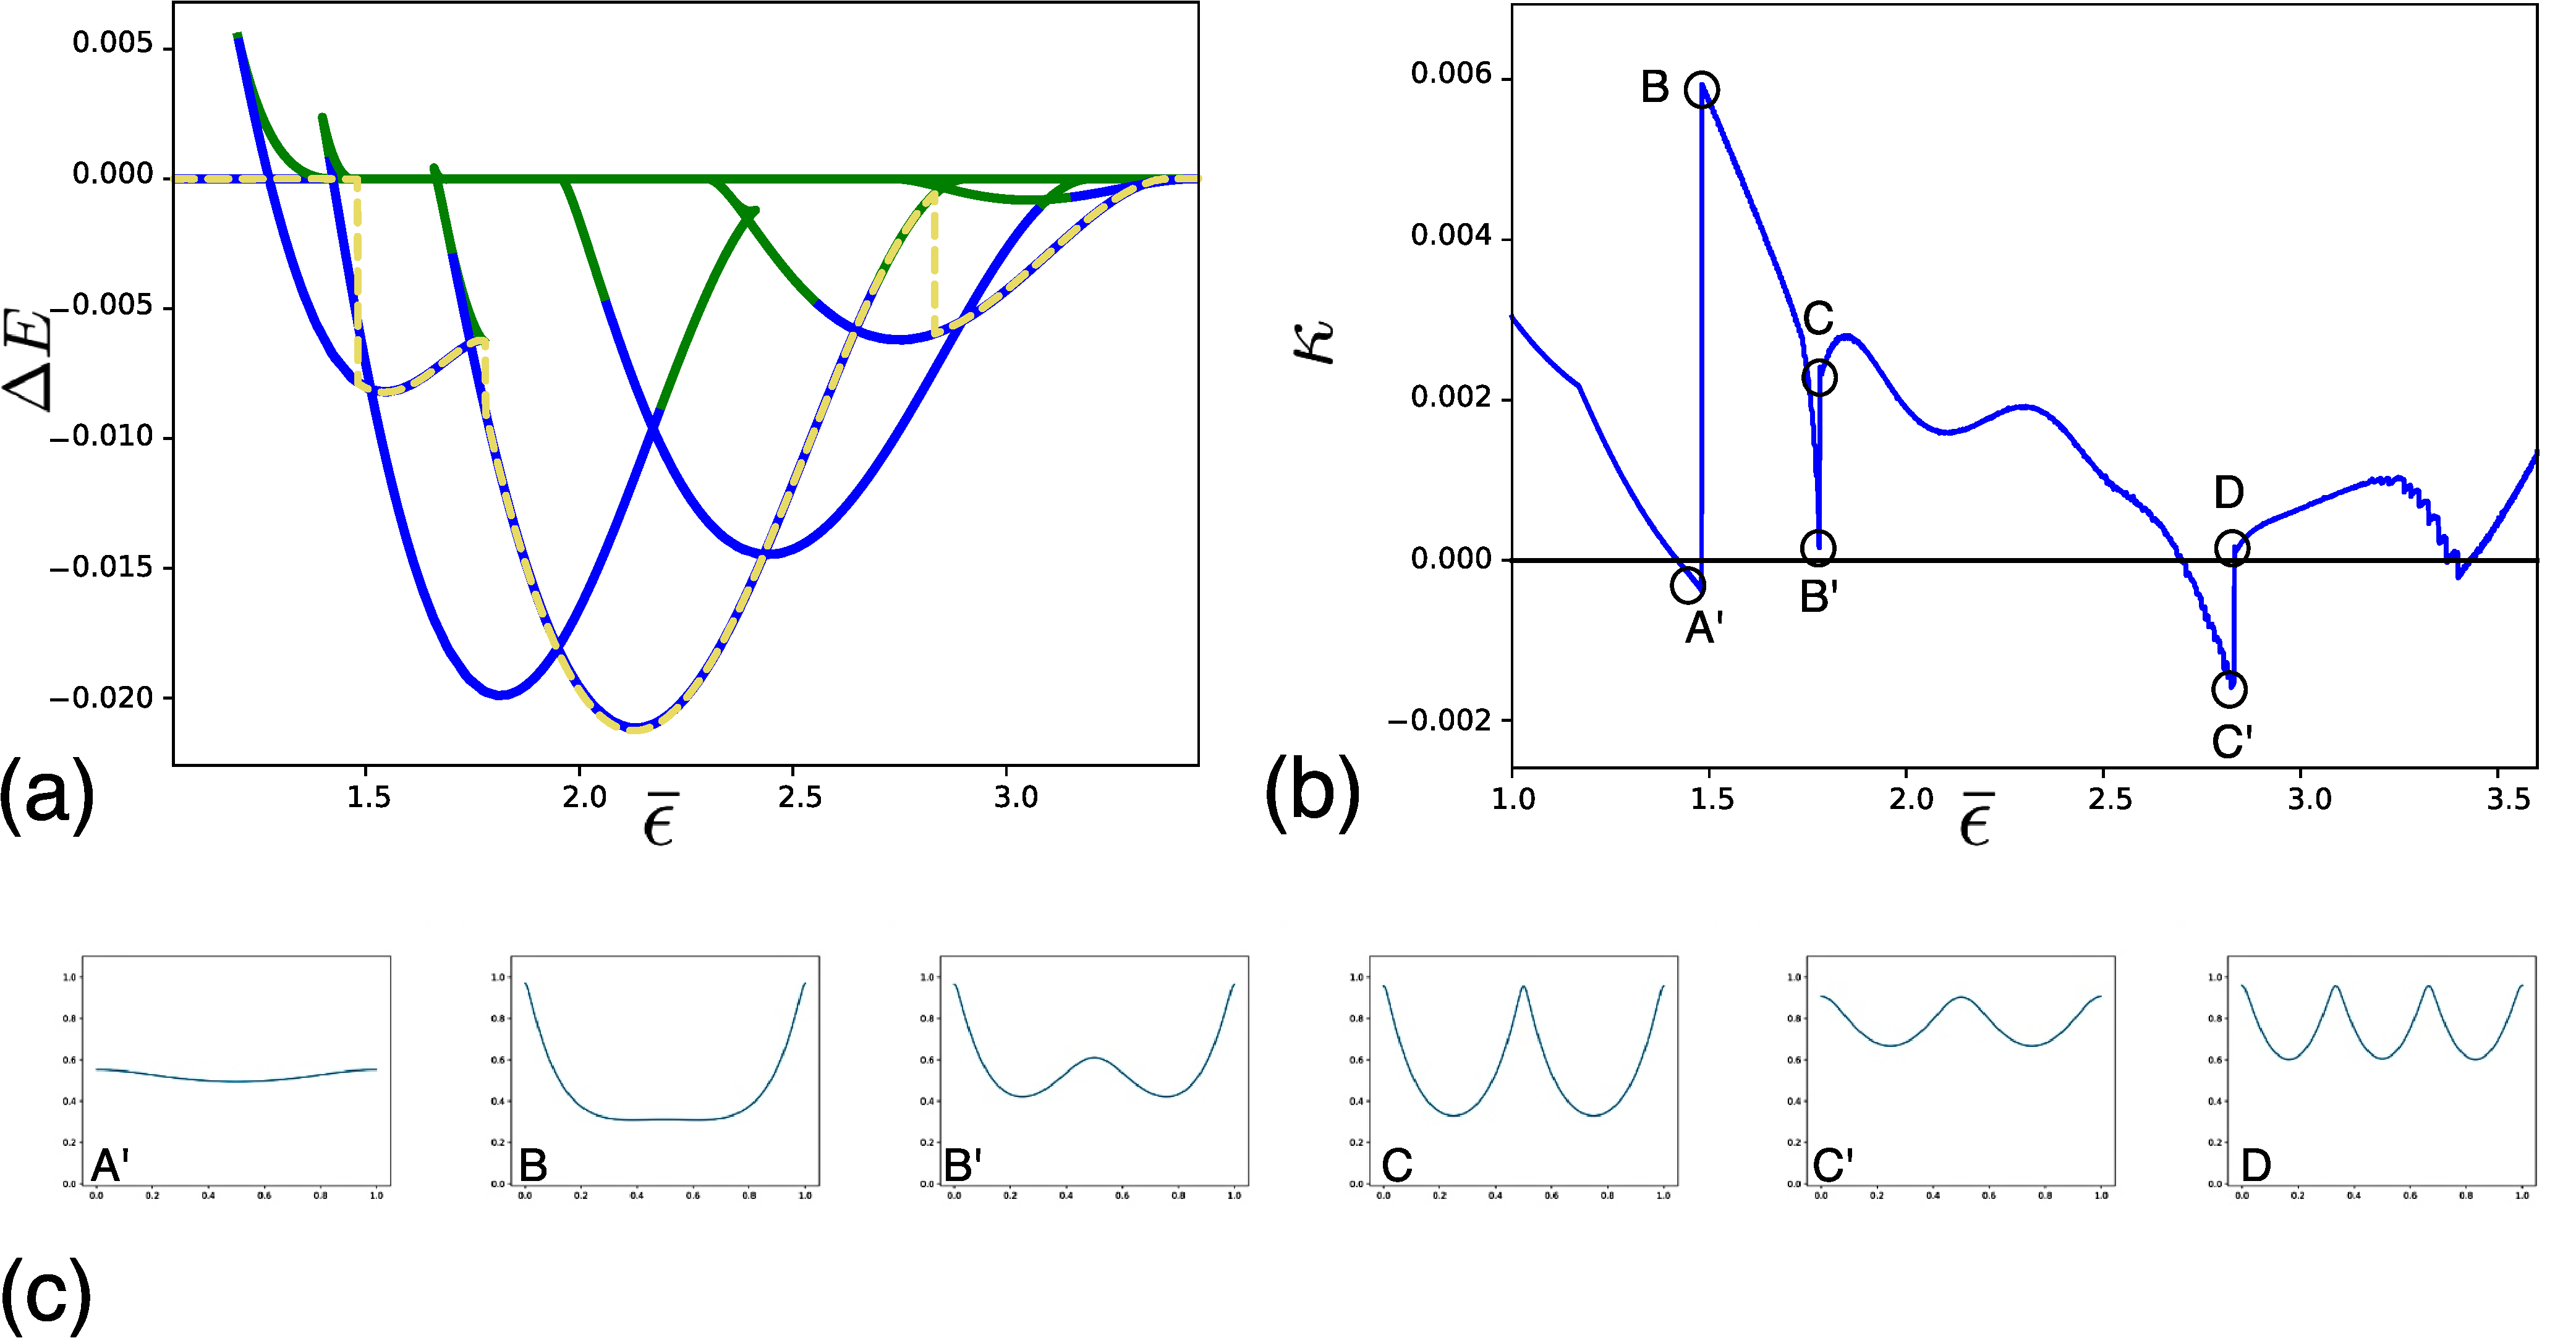
\includegraphics[scale=0.23]{final_images/fig5.pdf}
    \caption{
        \todo[inline]{Add marker for $\ep_c, H$ in Fig (a) and (b),
        add $n=3, 4, ...$ in Fig (a),
        add $n=3, 4, ...$ in Fig (c)
        }
        Quasi-static loading simulations with L-BFGS: (a) the energy difference $\Delta E$, between the quasi-Newton solutions and the homogeneous solutions are superimposed onto equilibrium branches (red); (b) smallest eigenvalue of the second variation  as a function of the loading parameter $\bar\epsilon$; (c) damage profiles.}
    \label{fig:tempo2}
\end{figure}


In our numerical experiments, we employ the BFGS and L-BFGS solvers from the Python SciPy library~\cite{2020SciPy-NMeth} and the Alglib library~\cite{Bochkanov2013-lk}. These solvers utilize the residual vectors (see \ref{residual1} and \ref{residual2}) at each finite element node, alongside the values of integrals \eqref{modeld} and \eqref{model_elastic_substrate}.
\begin{figure}
    %\centering
\includegraphics[width=\textwidth]{./final_images/fig6.pdf}
    \caption{
\todo[inline]{Fix legend colours in (a)}
Kick algorithm for the first model: (first column) the current unstable solution  for the damage field \added[id=ALB]{(blue)}, the \added[id=ALB]{eigenvector associated to the} smallest \replaced[id=ALB]{eigenvalue}{eigenvector} of this state \added[id=ALB]{(orange)}, and the perturbed damage field with this eigenvector \added[id=ALB]{(green)}; (second column)  the solution returned by the quasi-Newton algorithm wherein initial guess is taken to be the perturbed damage field.
 }
    
    \label{fig:kick}
\end{figure}


\begin{figure}
    %\centering
\includegraphics[width=\textwidth]{./final_images/fig7.pdf}
    \caption{Kick algorithm for the second model: (first column) the current unstable solution  for the damage field, the smallest eigenvector of this state, and the perturbed damage field with this eigenvector; (second column)  the solution returned by the quasi-Newton algorithm wherein initial guess is taken to be the perturbed damage field.
 }
 \label{fig:kick2}
\end{figure}

%To summarize, we initially provide the algorithms with an initial guess for $\mathbf{X}^{(k)} = (\mathbf{u}^{(k)}, \alpha^{(k)})$ at a fixed value of the loading parameter $\bar\epsilon$. Additionally, we specify an initial guess for the Hessian matrix, denoted as $\mathbf{B}^{k} \in \mathbb{R}^{n \times n}$. This matrix can either be set as the identity matrix or the uncoupled stiffness matrix to ensure a symmetric and positive definite approximation. Subsequently, the quasi-Newton algorithm computes a search direction using  the analogue of the Newton equation $\mathbf{B}^{(k)} \mathbf{p}^{(k)}  = -\mathbf{R}^{(k)} $,where $\mathbf{p}^{(k)}$ denotes the search direction at stage $k$. Afterwards, it  performs a line search to minimize a function $f(h^{(k)}) = f(\mathbf{X}^{(k)} + h^{(k)} \mathbf{p}^{(k)})$ in order to find an acceptable step size $h^{(k)}$ such that $h^{(k)} \in \arg \min_{h} f$. The solution is then updated in the direction of $\mathbf{p}^{(k)}$ with the step size $h^{(k)}$. 


In Figure \ref{fig:tempo1}(a), we present the results of our numerical experiments, overlaying solutions obtained from the quasi-Newton algorithm onto equilibrium branches determined using the pseudo-arclength continuation method described in the previous section. We show the stability of the solution in  Fig. \ref{fig:tempo1}(b), where it is clear that all the branch switching events are delayed in the sense they do not  take place when the smallest eigenvalue of the second variation vanishes but \comment[id=ALB]{only beyond the load corresponding to the eigenvalue's sign transition.}. Notably, the expected first branch switching event—from the trivial solution to the branch with \(n=3\) due to loss of stability as outlined in the LEM protocol—did not occur at point H as anticipated. Initially, it appears that the system remains on the trivial branch, as shown in Fig. \ref{fig:enter-label}(a), until it transitions to the branch with \(n=4\) at much higher values than the critical loading parameter \(\bar{\epsilon}^c\). By monitoring the smallest eigenvalue of the second variation of the solution, we observe that the quasi-Newton solutions become unstable beyond \(\bar{\epsilon}^c\), which is consistent for the trivial branch. However, closer inspection reveals that the quasi-Newton solutions are not homogeneous but instead exhibit the instability mode calculated analytically (or  the eigenvector associated with the smallest eigenvalue). For instance, the  quasi-Newton solution before the first branch switching event is shown in inset (A') in Fig. \ref{fig:tempo1}(b), where we see that \added[id=ALB]{the equilibrium damage shows a slight oscillation } reminiscent of the eigenmode \(\alpha_n(x) \sim \cos(n\pi x)\), \comment[id=ALB]{$\alpha_n(x) \sim c+ \cos(n\pi x)$ where $c$ is an arbitrary constant and} with \(n=3\) \textbf{what does it mean?}. On the other hand, the selected branch  by the quasi-Newton method is the one with \(n=4\) with one bulk crack and two boundary cracks, see inset (B) in Fig. \ref{fig:tempo1}(b). If the transition had taken place at \(\bar{\epsilon}^c\) as anticipated by our LEM strategy, the system would have reached a configuration with two bulk cracks and one boundary crack, as shown in Fig. \ref{fig:enter-label}(b) inset (A).

With continued loading, the damage increases, and the system evolves along this branch beyond the loading parameter value at which it first became unstable, as shown in Fig. \ref{fig:tempo1}(b). A dissipative branch switching event takes place from the current branch (\(n=4\)) at point \(B'\) to the branch with \(n=6\); see Fig. \ref{fig:tempo1}(b) inset C for the corresponding damage profile. The delay in bifurcation results in a different branch selection event than the one in our LEM protocol. Finally, we conclude that the delays at bifurcation for the first and second branch switching events leads to a completely different path compared to our LEM protocol until it finally reconnects with the homogeneous branch at point \(C'\).

After thoroughly dissecting the outcomes of the first mathematical model, we now transition to exploring the simulation results of the second model. The solutions of our  numerical experiments obtained from the quasi-Newton algorithm (gray dashed line) are overlaid onto equilibrium branches in Fig. \ref{fig:tempo2}(a), while their stability  is depicted in Fig. \ref{fig:tempo2}(b). Notably, we observe a delay, albeit less pronounced compared to the first model, for the bifurcation from the trivial branch, occurring at a higher value than the analytically determined critical value of the loading parameter \(\bar{\epsilon}^c\). Interestingly, the quasi-Newton method switches to the branch with $n=2$, which exhibits lower energy compared to the branch with $n=3$. This occurs  despite the delay in bifurcation because the branch  $n=3$ remains accessible for the current value $\bar\epsilon$. It's worth noting that our LEM protocol also anticipated a first branch selection event leading to the branch with $n=2$ with 2 boundary cracks. 
We again observe that, \added[id=ALB]{even before the first branch-changing event}, the quasi-Newton solution \replaced[id=ALB]{is an homogeneous state perturbed by an oscillatory term of}{deviates from the trivial branch, and the damage profile has} the form \(\sim \cos(n\pi x)\), reminiscent of the eigenmode $\alpha_n$ \comment[id=ALB]{$\alpha_n(x) \sim c+ \cos(n\pi x)$ where $c$ is an arbitrary constant and} with \(n=2\) \textbf{what does it mean?}. 
% \added[id=ALB]{Remark: this may be due to the quasi-Newton computation which necessarily relies on an approximate positive-definite Hessian. EXPAND}
\added[id=ALB]{These perturbations of the equilibrium profiles are negligible from the energetic standpoint, as it can be inferred in Figure~\ref{fig:tempo2}(a), by the superposition between the energy of the computed evolution and the exact total energy of the homogeneous solution.} 
When the branch with $n=2$ terminates, the minimization brings the system to the branch with $n=4$ although the branch with $n=3$ is also accessible and has lower energy, In Figure~\ref{fig:tempo2}(c), the corresponding damage profiles before and after \added[id=ALB]{the branch} switching event  at points B' and C. The final \replaced[id=ALB]{transition}{event} before the connection to the trivial branch takes place at point C', which is also an unstable configuration. The minimization brings the system to the branch with $n=6$ as seen in Fig. \ref{fig:tempo2}(b) and the corresponding stable damage profile at point D is shown in Fig. \ref{fig:tempo2}(c). 

In summary, while the results of the quasi-Newton minimization simulations exhibit overall similarities in both models, the trajectory taken by the system in the second model closely aligns with the LEM protocol outlined above. This alignment can be attributed to the specific energy landscape within the second model.

%: the states accessible to the system when the smallest eigenvalue vanishes remain unchanged compared to when the "delayed" branch switching occurs.

\subsection{Hybrid algorithm}
Our investigation reveals that the solutions generated by the quasi-Newton algorithms deviate from the prescribed LEM protocol outlined in the preceding sections. We observed a delayed bifurcation phenomenon and the presence of unstable solutions, \replaced[id=ALB]{both affecting}{affect} the branch selection events along the evolution.  This is indeed related to the fact that the energy landscape becomes extremely flat when the determinant Hessian gets close to zero~\textbf{comment more}
\added[id=ALB]{An energy expansion for a generic admissible state $y$ in the vicinity the fundamental equilibrium branch $y_t=(tx, \alpha_t)$ reads}  
$$
\Psi(y)-\Psi(y_t)= \delta\Psi(y_t)(y-y_t)+\frac{1}{2}(y-y_t)^T \delta^2\Psi(y_t)(y-y_t)+o(\|y-y_t\|^2)
$$

\added[id=ALB]{where $y$ verifies kinematic boundary conditions and its damage component $\alpha$ is either unconstrained or such that $\alpha\geq\alpha_t$, if irreversibility is taken into account. Along a the direction of a bifurcation mode, that is setting $y-y_t=h w_n$, where $w_n:=(v_n, \alpha_n)(x)$ is the $n$-th eigenmode associated to the Hessian, we obtain}

$$
\Psi(y)-\Psi(y_t)= \frac{h^2}{2}\lambda^2_n \|w_n\|^2+o(h^2\|w_n\|^2).
$$
\added[id=ALB]{The first order term $\delta\Psi(y_t)(v_n, \alpha_n)$ vanishes identically owing to the fact that the bifurcation mode is an admissible field for the equilibrium condition. This implies that, when the smallest eigenvalue continuously approaches zero, the energy landscape passes from being  locally convex and locally flat (at first order) in all admissible directions which include (in particular) the directions associated to the eigenmodes, to loosing local convexity in one non-trivial direction which is, in the numerical practice, shielded by the quasi-Newton approximation of the Hessian, necessary to guarantee the convergence of the numerical scheme. This can justify the systematic (and algorithm-dependent) delay of the bifurcation events via the quasi-Newton solver.}
To address this challenge, we introduce a hybrid approach. In this method, we continuously monitor the smallest eigenvalue of the complete \replaced[id=ALB]{Hessian}{stiffness} matrix for the equilibrium solutions obtained from the quasi-Newton algorithm. 
When this eigenvalue significantly diminishes, indicating potential instability, we calculate the corresponding eigenvector, denoted as \(\mathbf{p}\). We then use this eigenvector to perturb the current solution $\mathbf{X^*}$. This perturbation sets the initial guess for the next minimization step in the quasi-Newton algorithm as $\mathbf{\tilde X}^{(0)} = \mathbf{X^*} + h \mathbf{p},
$ where \(h\) is the step size.\comment[id=ALB]{I removed the k indices}
% \comment[id=ALB]{Does $k$ refer to the quasi-Newton iteration number? I think it can be removed}
This step size can, in principle, be determined through a line-search algorithm by minimizing the function $f(h) = \Psi(\mathbf{X} + h \mathbf{p})$ to find an optimal value \(h\), such that $h \in \arg \min_{h} f$. Instead, we \deleted[id=ALB]{initially}  set \(h = 1\)  (this choice is further discussed in the following) \added[id=ALB]{and run the quasi-Newton step to obtain a new critical point $\mathbf{\tilde X}$.}

We first discuss the outcome of this hybrid algorithm for the three anticipated branch-switching events identified for the first model previously reported in Fig. \ref{fig:enter-label}. For each of these three cases, the snapshots of the damage fields, the associated smallest eigenvectors \(\mathbf{p}\), \deleted[id=ALB]{and} the perturbed states \(\mathbf{\tilde X}^{(0)}\), and the converged solutions $\mathbf{\tilde X}$ are shown in Figs. \ref{fig:kick}(a,c,e).

When the quasi-Newton algorithm is initiated using the perturbed state \(\mathbf{\tilde X^{(0)}}\)
% \comment[id=ALB]{shouldn't the perturbed state read \(\mathbf{X}\)?} 
as the initial guess, bifurcation occurs in each case, and the final solutions returned from the quasi-Newton minimization are shown in Figs. \ref{fig:kick}(b,d,f). For the first case, which corresponds to the bifurcation from the trivial branch, the smallest eigenmode has the form of \(\cos(n\pi x)\) with \(n=3\), as identified through the linear stability analysis (see Fig. \ref{fig:kick}(a)). The quasi-Newton minimization returns a state with two boundary cracks and one interior crack, as shown in Fig. \ref{fig:kick}(b), which is the same as the solution found using the arc-length continuation algorithm that corresponds to the branch with \(n=3\) (see Fig. \ref{fig:enter-label}(b), inset A).  The hybrid algorithm is also successful in capturing the next two  anticipated branch   switching events: from the  branch with \(n=3\)  to the branch  with \(n=4\) (see Fig. \ref{fig:kick}(d)) and  from branch with \(n=4\)  to the branch  with \(n=5\) (see Fig. \ref{fig:kick}(f)).   We  conclude here that the hybrid algorithm is able to capture the unique path dictated by the LEM protocol shown in Fig. \ref{fig:enter-label}.   

We now continue our numerical investigations by focusing on the second model. In this case, according to the LEM protocol, the path through which the system may evolve under quasi-static loading is not unique due to the multiplicity of the solutions for  the given critical loads, i.e., external strain at which the stability of a branch is lost,  and, will be determined by the minimization algorithm. Note that this is not the case for the first model wherein there is a single equilibrium branch accessible to the system for all given critical loads. On the other hand, despite the fact that quasi-Newton algorithm was able to reproduce one of the possible paths predicted by the LEM protocol for the second model, the optimal path  may be different due to the delays in anticipated bifurcations. 


The system's response under the hybrid algorithm is depicted in Fig. \ref{fig:kick2}. The first column displays the perturbed damage profiles, while the second column shows the outcomes of the energy minimization process starting from  this perturbed state. Initially, a stable state with two nucleated boundary cracks (branch \( n=2 \)) is achieved following the destabilization of the trivial branch, as illustrated in Fig. \ref{fig:kick2}(b). Subsequently, an interior crack nucleates in the middle of the system (branch \( n=4 \)), as shown in Fig. \ref{fig:kick2}(d). The third event involves a transition from branch \( n=3 \) to branch \( n=5 \). The final event depicted in Fig. \ref{fig:kick2} is the transition to branch \( n=6 \). We do not illustrate the last  event before reconnecting to the trivial branch since it is the only available branch to the system at this load, which is the transition from branch \( n=6 \) to branch \( n=7 \). To summarize, the branches selected by the hybrid algorithm follow the sequence 
\( 0 \rightarrow 2 \rightarrow 3 \rightarrow 5 \rightarrow 6 \rightarrow 7 \rightarrow 0 \), 
which differs from the sequence 
\( 0 \rightarrow 2 \rightarrow 3 \rightarrow 4 \rightarrow 6 \rightarrow 7 \rightarrow 0 \) 
followed by the quasi-Newton algorithm.

Finally, we will discuss the determination of the step-size \( h \) used to obtain the perturbed state as the initial guess for the quasi-Newton algorithm.
Typically, an optimal value for the step-size can be found by minimizing the function defined as \( f(h) := \Psi(\mathbf{X} + h \mathbf{p}) \).\comment[id=ALB]{This is said twice} However, in our case, the smallest eigenvalue of the system's Hessian is slightly less than zero, resulting in a very small \( h \) that prevents the quasi-Newton algorithm from escaping the flat region of the energy landscape.

To effectively escape this region, one can design an iterative algorithm that repeatedly performs line searches in the current unstable direction followed by minimization, iteratively flowing along the escape path. However, for the current problem, it was sufficient to take the step-size \( h=1 \) to escape the unstable state that solves the first-order problem \( \delta \Psi=0 \), even though our choice increases the function \( f(h) \). Indeed, the essential feature of the quasi-Newton algorithm is the positive definiteness of the approximate Hessian, independent of the function's curvature (positive or negative). Consequently, the quasi-Newton direction will always be a descent direction. Therefore, the perturbed state obtained by taking a large step-size moves the system away from the flat region, allowing the quasi-Newton algorithm to find the next lower energy branch. It remains to be seen if this choice will work in other models or more elaborated algorithm as suggested above has to be implemented, which will be the subject of future work.

\subsection{\added[id=ALB]{The role of irreversibility} }

To conclude this contribution, 
we qualitatively discuss the evolution which solves the full stability problem~\eqref{} of an initially undamaged thin film on a stiff substrate undergoing homogeneous evolution, highlighting the role of the irreversibility constraint on the global definition of space of perturbations.
Pointwise, the irreversibility constraint restricts branch switching events in such a way that, e.g., the transition between branches with $n=3$ and $n=4$  (cf. profiles in the figure \ref{fig:kick2} of the transition (d)$\mapsto$ (f) (CHECK)) is not allowed, as it requires a local decrease of the damag field. On the other hand, irreversibility as global constraint on the perturbation space renders the analysis more involed, as the additional requirement makes the problem strongly singular/nonlinear.

% The former is determined by the smallest eigenvalue of the operator $H(y)$, which is a non-linear operator that depends on the current damage state, whereas the latter is determined by the eigenvalue problem in the vector space.
We perform a one-dimensional test using the same parameters as in the experiment~\ref{..} for the rigid substrate model, plotting in Figure~\ref{fig:irreversibility}-top the profiles of the fields at the two loading steps corresponding with points X and Y in Figure~\ref{}.
More precisely, we plot the film displacement $u$ (linear and coincididing with the substrate's displacement) and the homogeneous damage field $\alpha_t$ alongside the profile of the eigenfunctions associated to the minimal eigenvalues both for the second order bifurcation~\eqref{eq:variational_inequality} (continuous black line) and for the stability problem~\eqref{eq:variational_stability}.
The bifurcation profiles coincide with the modes $n=4, 5$ alredy found, cf.~\eqref{} and are computed at two loads $t_b < t_1 < t_2$. 
Note that the profiles of the instability modes do not reduce to a truncation (i.e. a projection on the cone $K^+_0$) of the bifurcation modes, due to the necessary continuity of first derivatives. 
In Figure~\ref{fig:irreversibility}-bottom, we plot the spectra of the Hessian operator for the bifurcation problem (with blue circles and red crosses) as well as the smallest eigenvalue in the cone-constrained problem (with green and red losanges). 
Note that the bifurcation spectrum is singular at $t=0$, which is due to the fact that, in this model, the evolution of damage starts as soon as $t>0$, whereas the first order inequality (damage criterion) is verified with a strict inequality at $t=0$, throughout the entire domain. The bifurcation problem is singular in the sense that the set of admissible damage perturbations changes from $\emptyset$ to the vector space $V_0$, whereas the stability problem is singular in the sense that the set of admissible perturbations changes from the empty set to the solid cone $\{\beta\in H^1((0,1)):\beta \geq 0\}$ at soon as $t>0$.
In the inset, we zoom on the infimum of the spectra which shows the transition from the uniqueness of the homogeneous branch to the existence, for $t \geq t_b$, of a multiplicity of equilibrium curves passing through the current homogeneous state.
Despite the occurrence of negative eigenvalues for the bifurcation problem, the numerical solution indicates that there exists a sequence of positive eigenvalues for the (cone-constrained) stability problem, which is a sufficient condition for the stability of the computed evolution. Note that eigenvalues of the stability problem are only computed for $t\geq t_b$, as the uniqueness of the evolution branch guarantees its stability for $t<t_b$.
% Put in perspective with previous JMPS artcle.

% An image of the eigenmode which was inadmissible, meaning nucleation does not occur at the critical load of the reversible model. After showing that, we can further discuss the localization of the first crack formation. 
% Alternatively, we could mention that the irreversible case is more complex and that branch selection requires separate work using the tools in your JMPS.


\begin{figure}[htbp]
    \centering
    \includegraphics*[width=.45\textwidth]{final_images/damage_profile-16.png}
    \includegraphics*[width=.45\textwidth]{final_images/damage_profile-19.png}\\
    \includegraphics*[width=.45\textwidth]{final_images/spectra-7f4361886184f3c6791fe16bf4f4b3f2.pdf}
    \includegraphics*[width=.45\textwidth]{final_images/spectra-zoom-7f4361886184f3c6791fe16bf4f4b3f2.pdf}
    \caption{(a) Profiles of optimal perturbations for the bifurcation and stability problems, (b) Spectra of the Hessian operator for the bifurcation (circles) and stability (losanges) problems. The detail of the inf of the spectra is shown in (c)}
    \label{fig:irreversibility}
\end{figure}\todo[]{Add markers, $t_b$}


